\documentclass[11pt,a4paper]{report}
\usepackage[spanish,es-nodecimaldot]{babel}	% Utilizar español
\usepackage[utf8]{inputenc}					% Caracteres UTF-8
\usepackage{graphicx}						% Imagenes
\usepackage[hidelinks]{hyperref}			% Poner enlaces sin marcarlos en rojo
\usepackage{fancyhdr}						% Modificar encabezados y pies de pagina
\usepackage{float}							% Insertar figuras
\usepackage[textwidth=390pt]{geometry}		% Anchura de la pagina
\usepackage[nottoc]{tocbibind}				% Referencias (no incluir num pagina indice en Indice)
\usepackage{enumitem}						% Permitir enumerate con distintos simbolos
\usepackage[T1]{fontenc}					% Usar textsc en sections
\usepackage{amsmath}						% Símbolos matemáticos
\usepackage{listings}

% Comando para poner el nombre de la asignatura
\newcommand{\asignatura}{Simulación de Sistemas}
\newcommand{\autor}{Vladislav Nikolov Vasilev}
\newcommand{\titulo}{PRÁCTICA 1}
\newcommand{\subtitulo}{Diferentes Modelos de Simulación}

% Configuracion de encabezados y pies de pagina
\pagestyle{fancy}
\lhead{\autor{}}
\rhead{\asignatura{}}
\lfoot{Grado en Ingeniería Informática}
\cfoot{}
\rfoot{\thepage}
\renewcommand{\headrulewidth}{0.4pt}		% Linea cabeza de pagina
\renewcommand{\footrulewidth}{0.4pt}		% Linea pie de pagina

\begin{document}
\pagenumbering{gobble}

% Pagina de titulo
\begin{titlepage}

\begin{minipage}{\textwidth}

\centering


\includegraphics[scale=0.5]{img/ugr.png}\\

\textsc{\Large \asignatura{}\\[0.2cm]}
\textsc{GRADO EN INGENIERÍA INFORMÁTICA}\\[1cm]

\noindent\rule[-1ex]{\textwidth}{1pt}\\[1.5ex]
\textsc{{\Huge \titulo\\[0.5ex]}}
\textsc{{\Large \subtitulo\\}}
\noindent\rule[-1ex]{\textwidth}{2pt}\\[3.5ex]

\end{minipage}

\vspace{0.5cm}

\begin{minipage}{\textwidth}

\centering

\textbf{Autor}\\ {\autor{}}\\[2.5ex]
\textbf{Rama}\\ {Computación y Sistemas Inteligentes}\\[2.5ex]
\vspace{0.3cm}


\includegraphics[scale=0.3]{img/etsiit.jpeg}

\vspace{0.7cm}
\textsc{Escuela Técnica Superior de Ingenierías Informática y de Telecomunicación}\\
\vspace{1cm}
\textsc{Curso 2018-2019}
\end{minipage}
\end{titlepage}

\pagenumbering{arabic}
\tableofcontents
\thispagestyle{empty}				% No usar estilo en la pagina de indice

\newpage

\setlength{\parskip}{1em}

\chapter{Mi primer modelo de Montecarlo}

\section{Pruebas iniciales con el modelo}

Inicialmente, se ha probado el modelo para ver cómo funcionaba. Se ha ejecutado el modelo una serie de
veces (10 para ser más precisos), y se han almacenado los resultados. Estos resultados pueden verse a
continuación:

\begin{table}[H]
\centering
\begin{tabular}{c|c}
\textbf{Mejor posición inicial ($c$)} & \textbf{Mejor distancia} \\ \hline
95                              & 6.525780                 \\
94                              & 6.472190                 \\
94                              & 6.513340                 \\
94                              & 6.531020                 \\
94                              & 6.498630                 \\
93                              & 6.512340                 \\
94                              & 6.469870                 \\
94                              & 6.487920                 \\
94                              & 6.486590                 \\
94                              & 6.478660                
\end{tabular}
\caption{Resultados de mejor posición inicial y mejor distancia para 10 ejecuciones.}
\label{aparc-tabla}
\end{table}

Como se puede apreciar, parece que hay cierta semejanza entre los resultados obtenidos en cada
ejecución. Se puede ver que el valor de $c$ obtenido es muy similar en casi todos los casos, siendo
la moda $c = 94$, y la media un valor muy próximo a éste. Los valores de la mejor distancia también
son muy próximos entre sí, ya que todos ellos rondan, aproximadamente, las 6.5 plazas. Por tanto, el
modelo es capaz de producir unos resultados muy similares a pesar de que utiliza cierta ``aleatoriedad''.

Si estudiamos cómo evoluciona el valor de la distancia al destino a medida que cambia el valor de $c$, nos
encontramos con la siguiente gráfica:

\begin{figure}[H]
\centering
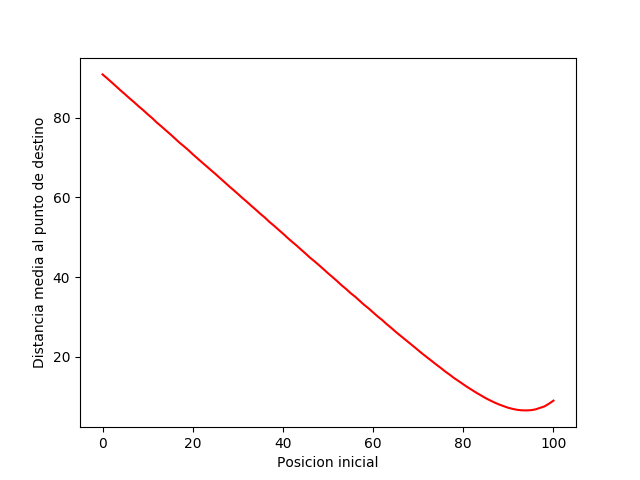
\includegraphics[scale=0.6]{img/c-dist.png}
\caption{Evolución del valor de la distancia al destino en función del valor de la posición inicial.}
\label{aparc-grafica}
\end{figure}

Como se puede ver, existe una tendencia a que, cuanto más cerca de la posición a la que se quiera llegar
se comienza a buscar sitio (es decir, cuanto más alto sea el valor de $c$), menor será la distancia hasta
el destino. Esto es completamente lógico, ya que al comenzar a buscar sitio a partir de una posición
muy lejana al destino, mayor será la distancia hasta éste en caso de que se encuentre una plaza libre. Teniendo
en cuenta que se escoge la primera plaza libre, ésta puede quedar muy lejos del destino, que es lo que se puede
apreciar en la gráfica.

El valor ideal de $c$, con las condiciones en las que estamos, parece ser $c = 94$. A partir de ahí, se puede ver
que existe un ligero incremento en la distancia al destino, posiblemente porque se aparque más lejos debido a que
no se encuentre una plaza libre en posiciones más cercanas al destino.

Por tanto, a vista de los resultados que hemos obtenido, podemos afirmar con bastante certeza que la plaza ideal
a partir de la que empezar sitio para aparcar es aproximadamente la 94.

\section{Experimentación con los parámetros}

Se han realizado una serie de experimentaciones con los parámetros con los que se puede llamar al programa.
A continuación, se muestran algunos de los resultados obtenidos.

\subsection{Modificación de la posición destino}

Se ha probado a modificar la posición destino, estableciendo que $x = 150$, y se han realizado 10 ejecuciones.
A continuación, se pueden ver los resultados obtenidos:

\begin{table}[H]
\centering
\begin{tabular}{c|c}
\textbf{Mejor posición inicial ($c$)} & \textbf{Mejor distancia} \\ \hline
144                              & 6.438900                 \\
144                              & 6.438900                 \\
144                              & 6.438900                 \\
143                              & 6.472200                 \\
143                              & 6.472200                 \\
143                              & 6.472200                 \\
143                              & 6.472200                 \\
143                              & 6.472200                 \\
143                              & 6.472200                 \\
143                              & 6.358800                
\end{tabular}
\caption{Resultados de mejor posición inicial y mejor distancia para 10 ejecuciones con
con posición destino $x = 150$.}
\label{aparc-150-tabla}
\end{table}

\begin{figure}[H]
\centering
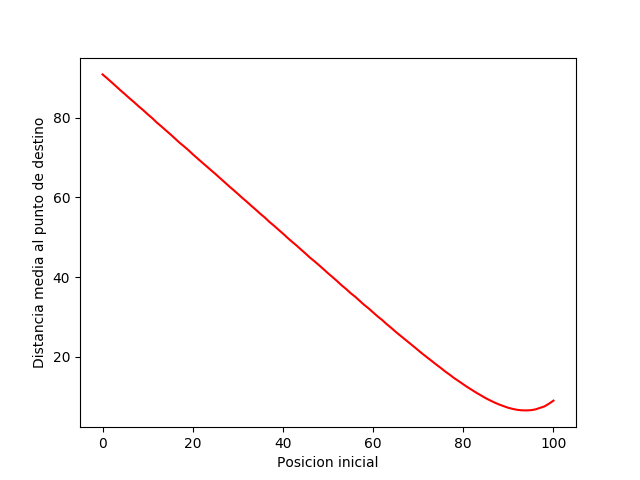
\includegraphics[scale=0.47]{img/c-dist.png}
\caption{Evolución del valor de la distancia al destino en función del valor de la posición inicial para $x = 150$.}
\label{aparc-150-grafica}
\end{figure}

Los resultados obtenidos en la tabla \ref{aparc-150-tabla} son muy parecidos a los que obtuvimos en \ref{aparc-tabla},
solo que los valores de $c$ han cambiado, aunque siguen unos patrones parecisos. En este caso, la moda parece ser 143,
y la media tiende a ese valor. Las mejores distancias están también muy próximas, y no se ve mucha disparidad.

Además, tal y como se hizo en el caso anterior, se ha obtenido una gráfica que muestra la evolución de la distancia media
en función del valor de $c$, la cuál se puede ver en la figura \ref{aparc-150-grafica}. Como se puede observar, sigue
un patrón muy parecido al que se puede ver en la figura \ref{aparc-grafica}, así que parece que no es un parámetro
que influya demasiado por sí solo.

\subsection{Modificación de la probabilidad de ocupación}

Se ha probado a variar la probabilidad de ocupación para ver cómo es afectada la salida. A continuación, se pueden ver
los resultados que se han obtenido:

\begin{table}[H]
\begin{tabular}{c|c|c}
\textbf{Probabilidad de ocupación} & \textbf{Mejor posición inicial} & \textbf{Mejor distancia} \\ \hline
0.01                               & 99                              & 0.008400                 \\
0.1                                & 99                              & 0.100000                 \\
0.2                                & 99                              & 0.213100                 \\
0.3                                & 99                              & 0.344800                 \\
0.4                                & 99                              & 0.495100                 \\
0.5                                & 98                              & 0.744800                 \\
0.6                                & 98                              & 1.074900                 \\
0.7                                & 98                              & 1.659600                 \\
0.8                                & 97                              & 2.901000                 \\
0.9                                & 94                              & 6.477300                 \\
0.99                               & 36                              & 67.957802               
\end{tabular}
\caption{Valores mejor posición inicial y distancia en función de la probabilidad de ocupación.}
\label{aparc-tabla-prob}
\end{table}

Es interesante ver cómo, a medida que va incrementando la probabilidad de ocupación, los valores de $c$ y de distancia
van cambiando, y se van haciendo cada vez peores. Se puede ver como el valor de $c$ va disminuyendo a medida que va aumentando
la probabilidad, lo cuál afecta directamente a la distancia, aumentándola proporcionalmente cada vez que disminuye el valor de
$c$. Todo esto se debe a que, cuanto menor sea la probabilidad de ocupación, más cerca del destino se podrá encontrar un sitio.
Todo esto se puede ver gráficamente en la siguiente figura:

\begin{figure}[H]
\centering
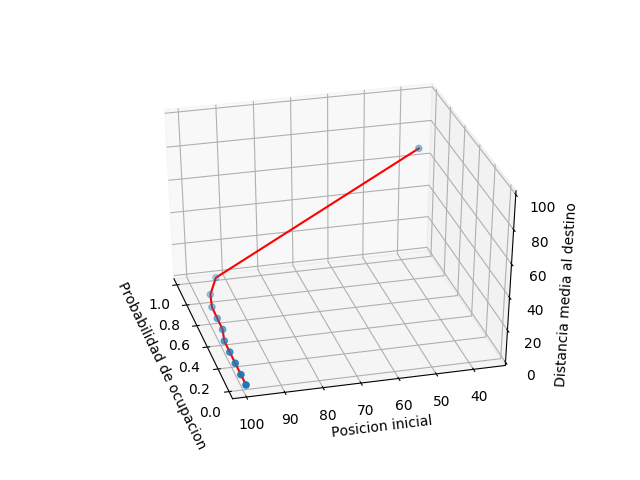
\includegraphics[scale=0.6]{img/aparc-prob-3d.png}
\caption{Representación 3D de la distancia media al destino en función de la probabilidad de ocupación y
la posición inicial.}
\label{aparc-3d-prob}
\end{figure}

Como se puede ver en la figura \ref{aparc-3d-prob},

Si se prueba con valores muy extremos, como por ejemplo con probabilidad de ocupación de 0.999, se obtiene el
siguiente error:

\begin{figure}[H]
\centering
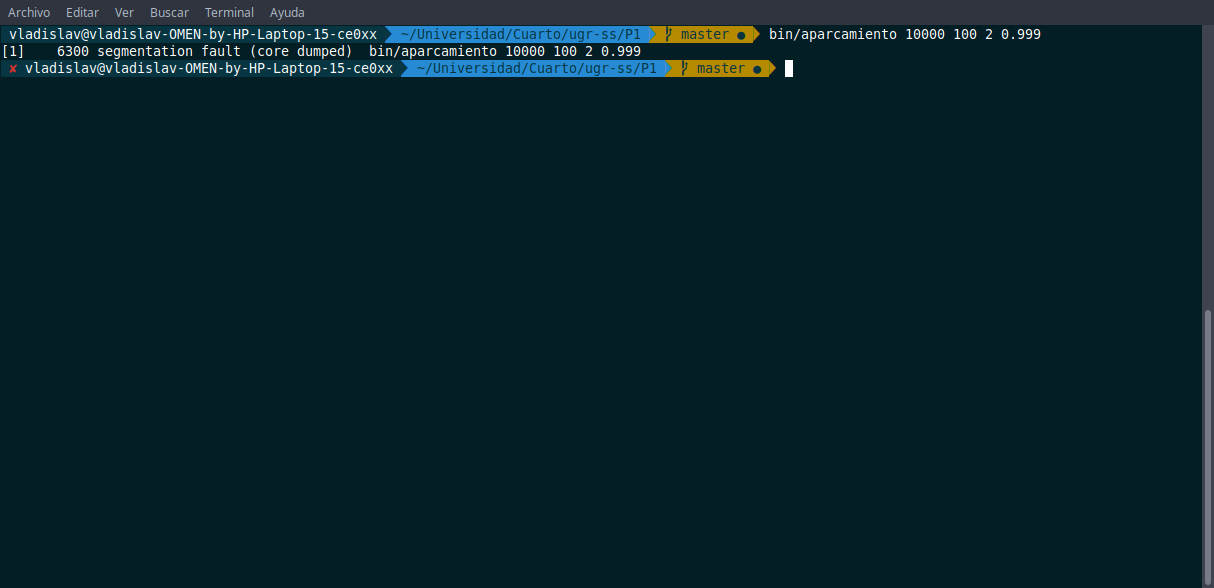
\includegraphics[scale=0.3]{img/aparc-prob-error.png}
\caption{Error al ejecutar el programa \textit{aparcamiento} con 0.999 de probabilidad de ocupación.}
\end{figure}


Esto se debe a que no se consigue encontrar sitio libre y se supera el tamaño del vector que representa las posiciones,
lo cuál genera un fallo de segmentación al intentar acceder a posiciones no válidas de memoria.

\subsection{Modificación del nivel de visión}

\newpage

\begin{thebibliography}{5}

\bibitem{nombre-referencia}
Texto referencia
\\\url{https://url.referencia.com}

\end{thebibliography}

\end{document}

